\documentclass{llncs}
\usepackage{times}
\usepackage[T1]{fontenc}

% Comentar para not MAC Users
%\usepackage[applemac]{inputenc}

\usepackage{a4}
%\usepackage[margin=3cm,nohead]{geometry}
\usepackage{epstopdf}
\usepackage{indentfirst}
\usepackage{graphicx}
\graphicspath{{Capturas-Ecra/}}
\usepackage{float}
\usepackage{fancyvrb}
\usepackage{amsmath}
\usepackage{array}
%\renewcommand{\baselinestretch}{1.5}


\begin{document}
\mainmatter
\title{TP1 - Protocolos da Camada de Transporte}

\titlerunning{TP1 - Protocolos da Camada de Transporte}

\author{Diogo Braga \and João Silva}

\authorrunning{Diogo Braga \and João Silva}

\institute{
University of Minho, Department of  Informatics, 4710-057 Braga, Portugal\\
e-mail: \{a82547,a82005\}@alunos.uminho.pt\\
PL2, Grupo 6
}

\date{}
\bibliographystyle{splncs}

\maketitle

\section{Questão 1}

\begin{center}
\begin{tabular}{ | m{3cm} | m{3cm} | m{3cm} | m{3cm} | m{3cm} |}
\hline
 \textbf{Comando usado (aplicação)} & \textbf{Protocolo de Aplicação(se aplicável)} & \textbf{Protocolo de transporte(se aplicável)} & \textbf{Porta de atendimento(se aplicável)} & \textbf{Overhead de transporte em bytes(se aplicável)} \\
 \hline
 \textbf{Ping} & -------------------------- & -------------------------- & -------------------------- & -------------------------- \\
 \hline
 \textbf{traceroute} & -------------------------- & -------------------------- & -------------------------- & -------------------------- \\
 \hline
 \textbf{telnet} & Telnet & TCP & 23 & 20 \\
 \hline
 \textbf{ftp} & FTP & TCP & 21 & 32 \\
 \hline
 \textbf{Tftp} & TFTP & UDP & 69 & 22 \\
 \hline
 \textbf{browser/http} & HTTP & TCP & 80 & 32 \\
 \hline
 \textbf{nslookup} & DNS & UDP & 53 & variável \\
 \hline
 \textbf{ssh} & SSH & TCP & 22 & 32 \\
 \hline
\end{tabular}
\end{center}

\subsection{Ping}

\begin{figure}[H]
\begin{center}
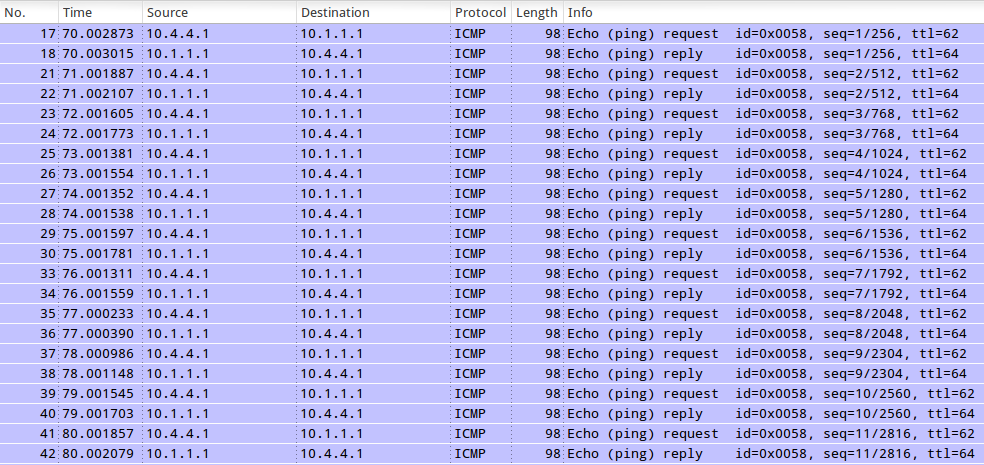
\includegraphics[scale=0.4]{ping.png}
\end{center}
\caption{\label{fig:ping}Captura realizada aquando a realização do comando \emph{ping}.}
\end{figure}

Como possível reparar na figura \ref{fig:ping}, o comando \emph{ping} apenas utiliza \textbf{ICMP} pelo que atua praticamente apenas no nível de rede, daí as nossas escolhas aquando do preenchimento do quadro.


\subsection{Traceroute}

\begin{figure}[H]
\begin{center}
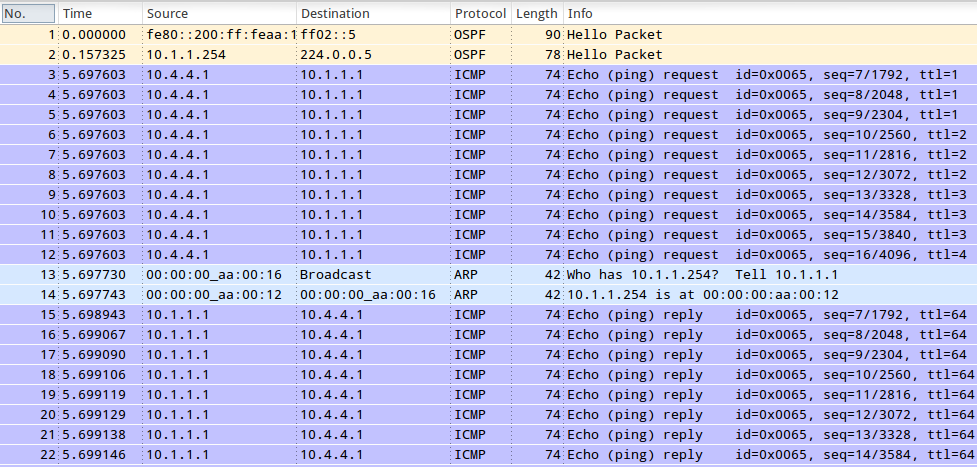
\includegraphics[scale=0.4]{traceroute.png}
\end{center}
\caption{\label{fig:traceroute}Captura realizada aquando a realização do comando \emph{traceroute}.}
\end{figure}

Como possível reparar na figura \ref{fig:traceroute}, o comando \emph{traceroute}, tal como o \emph{ping}, apenas utiliza \textbf{ICMP} pelo que atua praticamente apenas no nível de rede, daí as nossas escolhas aquando do preenchimento do quadro.


\subsection{Telnet}

\begin{figure}[H]
\begin{center}
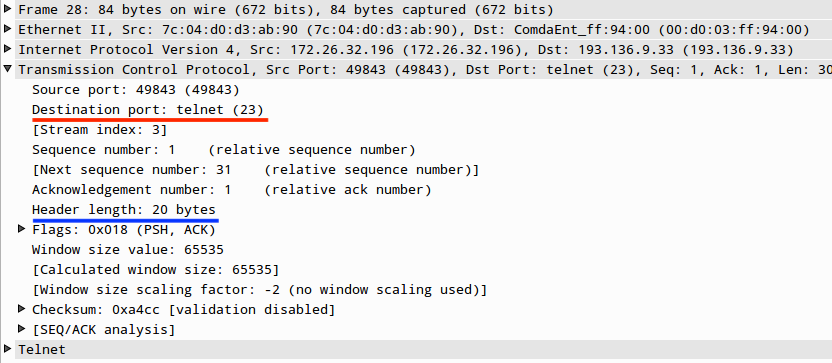
\includegraphics[scale=0.4]{telnet.png}
\end{center}
\caption{\label{fig:telnet}Captura realizada aquando a realização do comando \emph{telnet}.}
\end{figure}

A figura \ref{fig:telnet}, representa um Frame capturado que contém um cabeçalho referente à aplicação \textbf{Telnet}. Deste modo na camada de transporte (TCP) conseguimos identificar a porta de atendimento bem como o overhead de transporte em bytes, que se encontram a sublinhado na figura \ref{fig:telnet}.


\subsection{FTP}

\begin{figure}[H]
\begin{center}
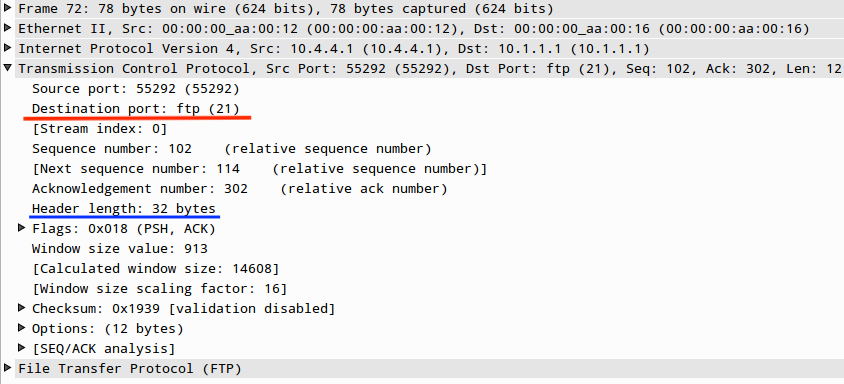
\includegraphics[scale=0.4]{ftp.png}
\end{center}
\caption{\label{fig:ftp}Captura realizada aquando a utilização do protocolo \emph{FTP}.}
\end{figure}

A figura \ref{fig:ftp}, representa um Frame capturado que contém um cabeçalho referente à aplicação \textbf{FTP}. Deste modo na camada de transporte (TCP) conseguimos identificar a porta de atendimento bem como o overhead de transporte em bytes, que se encontram a sublinhado na figura \ref{fig:ftp}.


\subsection{TFTP}

\begin{figure}[H]
\begin{center}
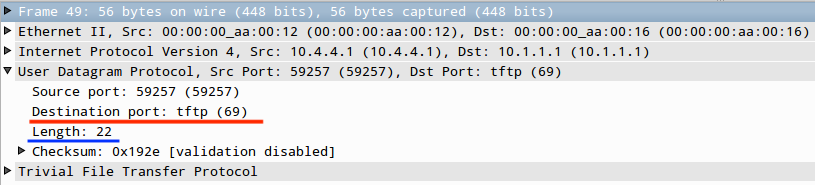
\includegraphics[scale=0.4]{tftp.png}
\end{center}
\caption{\label{fig:tftp}Captura realizada aquando a utilização do protocolo \emph{TFTP}.}
\end{figure}

A figura \ref{fig:tftp}, representa um Frame capturado que contém um cabeçalho referente à aplicação \textbf{FTP}. Deste modo na camada de transporte (UDP) conseguimos identificar a porta de atendimento bem como o overhead de transporte em bytes, que se encontram a sublinhado na figura \ref{fig:ftp}.


\subsection{HTTP}

\begin{figure}[H]
\begin{center}
\includegraphics[scale=0.4]{http.png}
\end{center}
\caption{\label{fig:http}Captura realizada aquando a utilização do protocolo \emph{HTTP}.}
\end{figure}

A figura \ref{fig:http}, representa um Frame capturado que contém um cabeçalho referente à aplicação \textbf{HTTP}. Deste modo na camada de transporte (TCP) conseguimos identificar a porta de atendimento bem como o overhead de transporte em bytes, que se encontram a sublinhado na figura \ref{fig:ftp}.


\subsection{Nslookup}

\begin{figure}[H]
\begin{center}
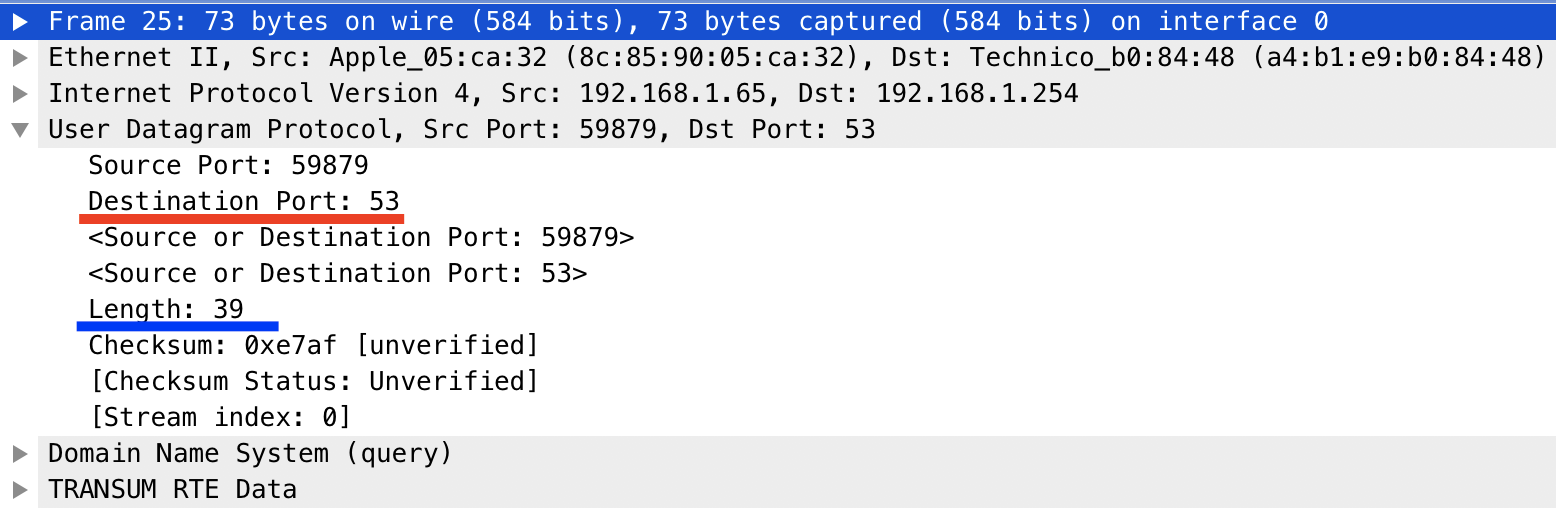
\includegraphics[scale=0.4]{nslookup.png}
\end{center}
\caption{\label{fig:nslook}Captura realizada aquando a utilização do comando \emph{nslookup}.}
\end{figure}

A figura \ref{fig:nslook}, representa um Frame capturado que contém um cabeçalho referente ao comando \textbf{nslookup}. Deste modo na camada de transporte (UDP) conseguimos identificar a porta de atendimento, já o overhead de transporte verificamos ser variável uma vez que mudava consoante as frames capturadas.



\subsection{SSH}

\begin{figure}[H]
\begin{center}
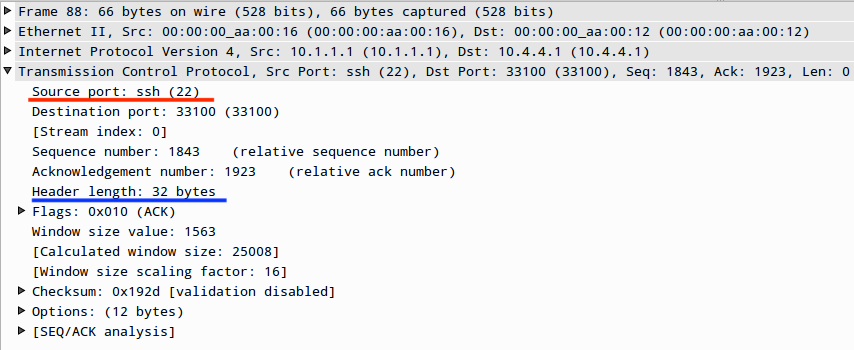
\includegraphics[scale=0.4]{ssh.png}
\end{center}
\caption{\label{fig:ssh}Captura realizada aquando a utilização do protocolo \emph{SSH}.}
\end{figure}

A figura \ref{fig:ssh}, representa um Frame capturado que contém um cabeçalho referente à aplicação \textbf{SSH}. Deste modo na camada de transporte (TCP) conseguimos identificar a porta de atendimento bem como o overhead de transporte em bytes, que se encontram a sublinhado na figura \ref{fig:ssh}.


\section{Questão 2}

Nas duas figuras seguintes, o endereço \textbf{10.1.1.1} identifica o \textbf{Servidor1} da LAN1, e o endereço \textbf{10.4.4.1} identifica o \textbf{Cliente1}, host da LAN4 da topologia em causa.

\begin{figure}[H]
\begin{center}
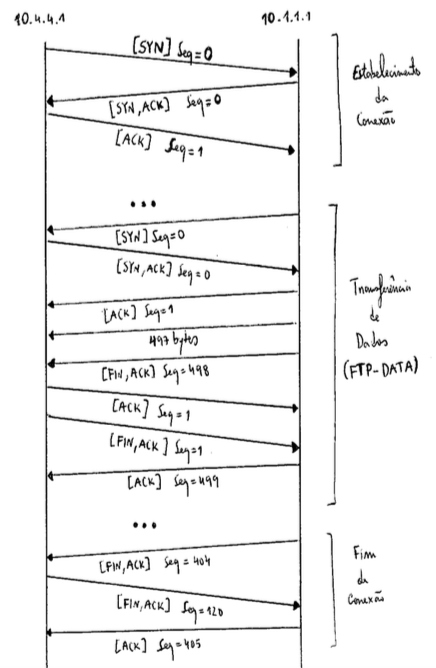
\includegraphics[scale=0.5]{2_ftp.png}
\end{center}
\caption{\label{fig:ssh}Diagrama temporal das transferências do file1 por \textbf{FTP}.}
\end{figure}

\begin{figure}[H]
\begin{center}
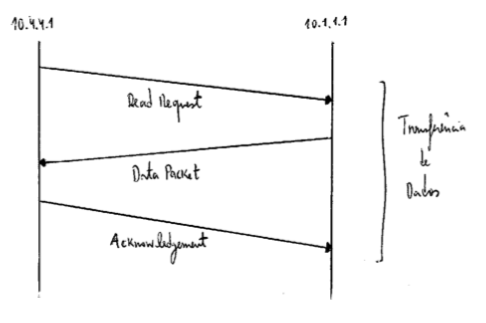
\includegraphics[scale=0.5]{2_tftp.png}
\end{center}
\caption{\label{fig:ssh}Diagrama temporal das transferências do file1 por \textbf{TFTP}.}
\end{figure}

\section{Questão 3}
\subsection{(i) uso da camada de transporte}
Perante os resultados obtidas na Questão 1, podemos concluir que, tanto o FTP, como o HTTP e o SSH utilizam o TCP como camada de transporte, enquanto o TFTP utiliza o UDP para essa função.

Isto leva-nos a concluir que no TFTP existe um menor controlo do envio dos dados por parte da camada de transporte, visto este ser antes controlado pela camada de aplicação.

Nas restantes aplicações em causa, como é usado o TCP sabemos que o transporte, sendo orientado à conexão, é realizado de uma forma mais fiável.

\subsection{(ii) eficiência na transferência}
No protocolo de aplicação TFTP, como é usado UDP, não há estabelecimento e terminação da conexão o que deixa menos garantias de que a transferência seja realizada com sucesso. Por outro lado o facto de não existirem estes \emph{handshakes}, torna a transferência do ficheiro muito mais eficiente.

Nos restantes três protocolos de aplicação, devido ao uso do TCP, a transferência é mais fiável, pois são efetuadas conexões lógicas, existindo em cada conexão um par de sockets. Este protocolo de transporte efetua também controlo de erros, de fluxo e de congestão, o que torna a transferência mais segura mas por outro lado, menos eficiente.

\subsection{(iii) complexidade}
Perante o observado, por exemplo na Questão 2, concluímos que a complexidade de usar UDP é consideravelmente inferior à de usar o TCP. No caso do TFTP conseguimos ver que apenas é realizada a transferência de dados relativos ao ficheiro.

Quanto ao uso de TCP, por exemplo no caso da utilização de FTP, é necessário estabelecer conexão entre o servidor e o cliente, enviar os dados relativos ao ficheiro, e por último desfazer a conexão. De referir ainda que estas fases de conexão e terminação de conexão são extensas e com várias trocas de segmentos entre ambos os participantes.

\subsection{(iv) segurança}
Quando dois sistemas comunicam sobre TCP, primeiramente necessitam de estabelecer conexão. Esta conexão é feita tendo em conta o IP origem, número de porta da origem, IP destino e número de porta destino, pelo que as comunicações entre estes dois sistemas são feitas unicamente por um socket, não podendo mais ninguém usar este para comunicar com o servidor. Fica desta forma mais difícil intercetar e enviesar comunicações. Este é o caso do FTP, SSH e HTTP.

Quanto às comunicações feitas sobre UDP, estas são identificadas através de dois números, o endereço IP destino, e número de porta destino. Como não se controlam as conexões, podem existir comunicações de qualquer equipamento, não havendo filtragem por porta nem IP, podendo desta forma ficar vulnerável a ataques alheios. Neste cenário encontra-se o TFTP.


\section{Questão 4}
No protocolo de aplicação TFTP, quando a transferência é executada a partir do Cliente1 tudo ocorre sem erros. Quando tal é executada a partir do Alfa, a porta do destino fica inalcançável, significando isto que foi detetado algum erro ... (ANALISAR BEM O WIRESHARK, TENHO DUVIDAS DISTO)



\section{Conclusões}

\end{document}
